\documentclass[12pt]{article}
%\usepackage[utf8]{inputenc}
%\documentclass[UTF8]{ctexart}
%\usepackage[UTF8, heading = false, scheme = plain]{ctex}
\usepackage{geometry}
%geometry{a4paper,scale=0.9}
\geometry{a4paper,left=1cm,right=1cm,top=1cm,bottom=2cm}
\usepackage{amsfonts}
\usepackage{color}
\usepackage{url}
%\usepackage{biblatex}
\usepackage{amsmath}
\usepackage{amssymb}
\usepackage{latexsym}
\usepackage{cite}
%\addbibresource{ref.bib}
%\bibliography{ref.bib}
\usepackage{caption}
\usepackage{graphicx, subfig}
\usepackage{float}
%\usepackage[fontset=ubuntu]{ctex}
%\usepackage{fontspec}
\usepackage{xeCJK}
%\usepackage[colorlinks,
%anchorcolor=black,
%citecolor=black]{hyperref}
%\setmainfont{SimSun}
\usepackage[section]{placeins}
\usepackage{enumitem}
\usepackage{framed}
\usepackage[framemethod=TikZ]{mdframed}
\usepackage{indentfirst}
\usepackage{setspace}%使用间距宏包
\linespread{1.5}
%\title{预备知识}
%\author{leolinuxer }
%\date{June 2020}

\title{深度学习中的 Product 层\cite{Product_Layer_In_Deep_Learning}}
\author{leolinuxer}
%\date{June 2020}

\begin{document}
\maketitle
\tableofcontents

\section{MLP 的特征交叉作用}
MLP(Multi-layer Perceptron)有对特征进行高阶交叉的作用,这是为什么?MLP中每个神经元不仅仅是对特征进行加权求和吗?

这个问题初看起来不能称之为一个问题,因为多层神经网络逼近任意函数都已经是理论证明过的工作了(Multilayer feedforward networks are universal approximators),用MLP去做特征交叉还不是轻而易举。但细想起来并不是那么简单。

大家都非常清楚,感知机的结构是一个基于加法操作的结构(下图),两个特征从来没有直接交叉过。即使到了下一层,不同特征之间,也不会直接相乘,而是继续以加权和的方式叠加起来。
\begin{figure}[H]
    \centering
    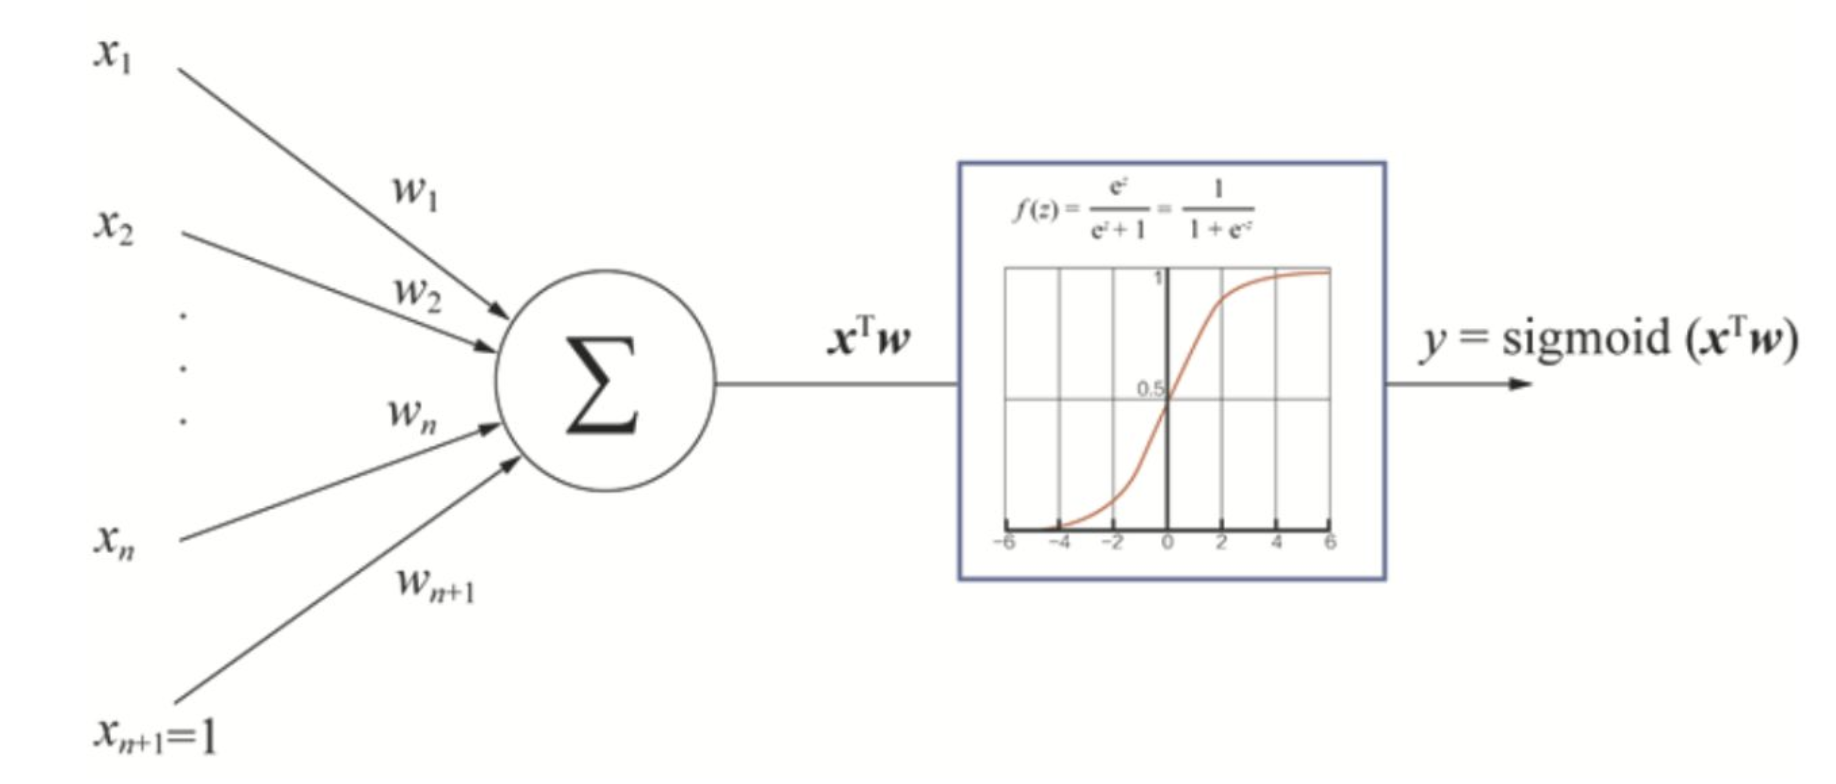
\includegraphics[width=.6\textwidth]{fig/Perception_Layer_Structure.png}
\end{figure}

那既然这样,为什么还说MLP具备特征交叉的能力呢?

就是\textbf{因为激活函数的存在,为MLP提供了非线性能力}。特征加权求和的结果,通过sigmoid,tanh这类激活函数之后,与其他神经元的输出进行进一步的混合,再通过下一层神经元的激活函数增加非线性,经过层层神经网络处理后,使MLP具备了特征交叉的能力,甚至在层数非常多之后,具备了拟合任意函数的能力。

但是,这里还是要强调的是,\textbf{MLP这种特征交叉的能力是比较弱的,MLP不是天生为了进行特征交叉设计的}。回到这篇文章标题中的话题,\textbf{这也就是为什么很多深度学习神经网络加入product层(特征乘积层)的原因}。

\section{Product 层}
我们来回顾一下那些加入了product层的知名的深度学习网络。

Google的Wide\&Deep模型中,Wide部分其实是两个特征的乘积层。
\begin{figure}[H]
    \centering
    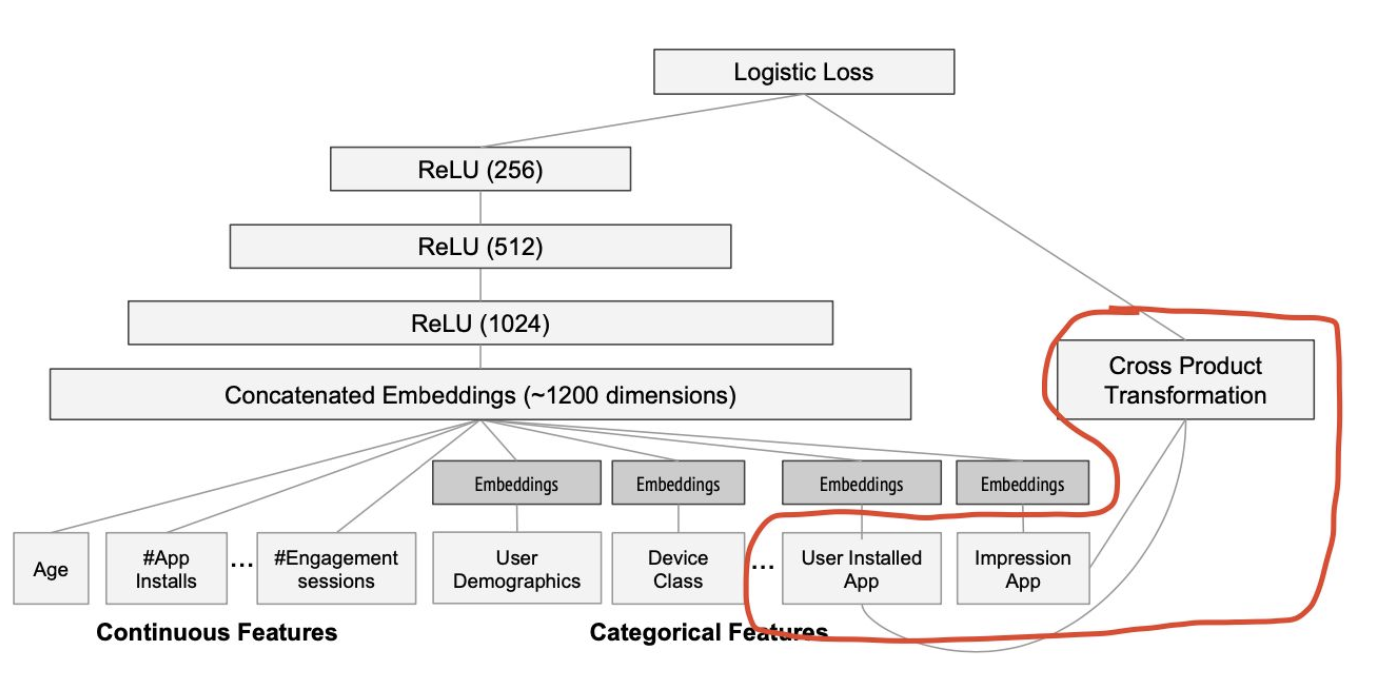
\includegraphics[width=1\textwidth]{fig/Wide_Deep_Structure_Detail.png}
\end{figure}

DeepFM中,用FM layer进行特征交叉,用MLP进行作为DeepFM中的Deep部分。
\begin{figure}[H]
    \centering
    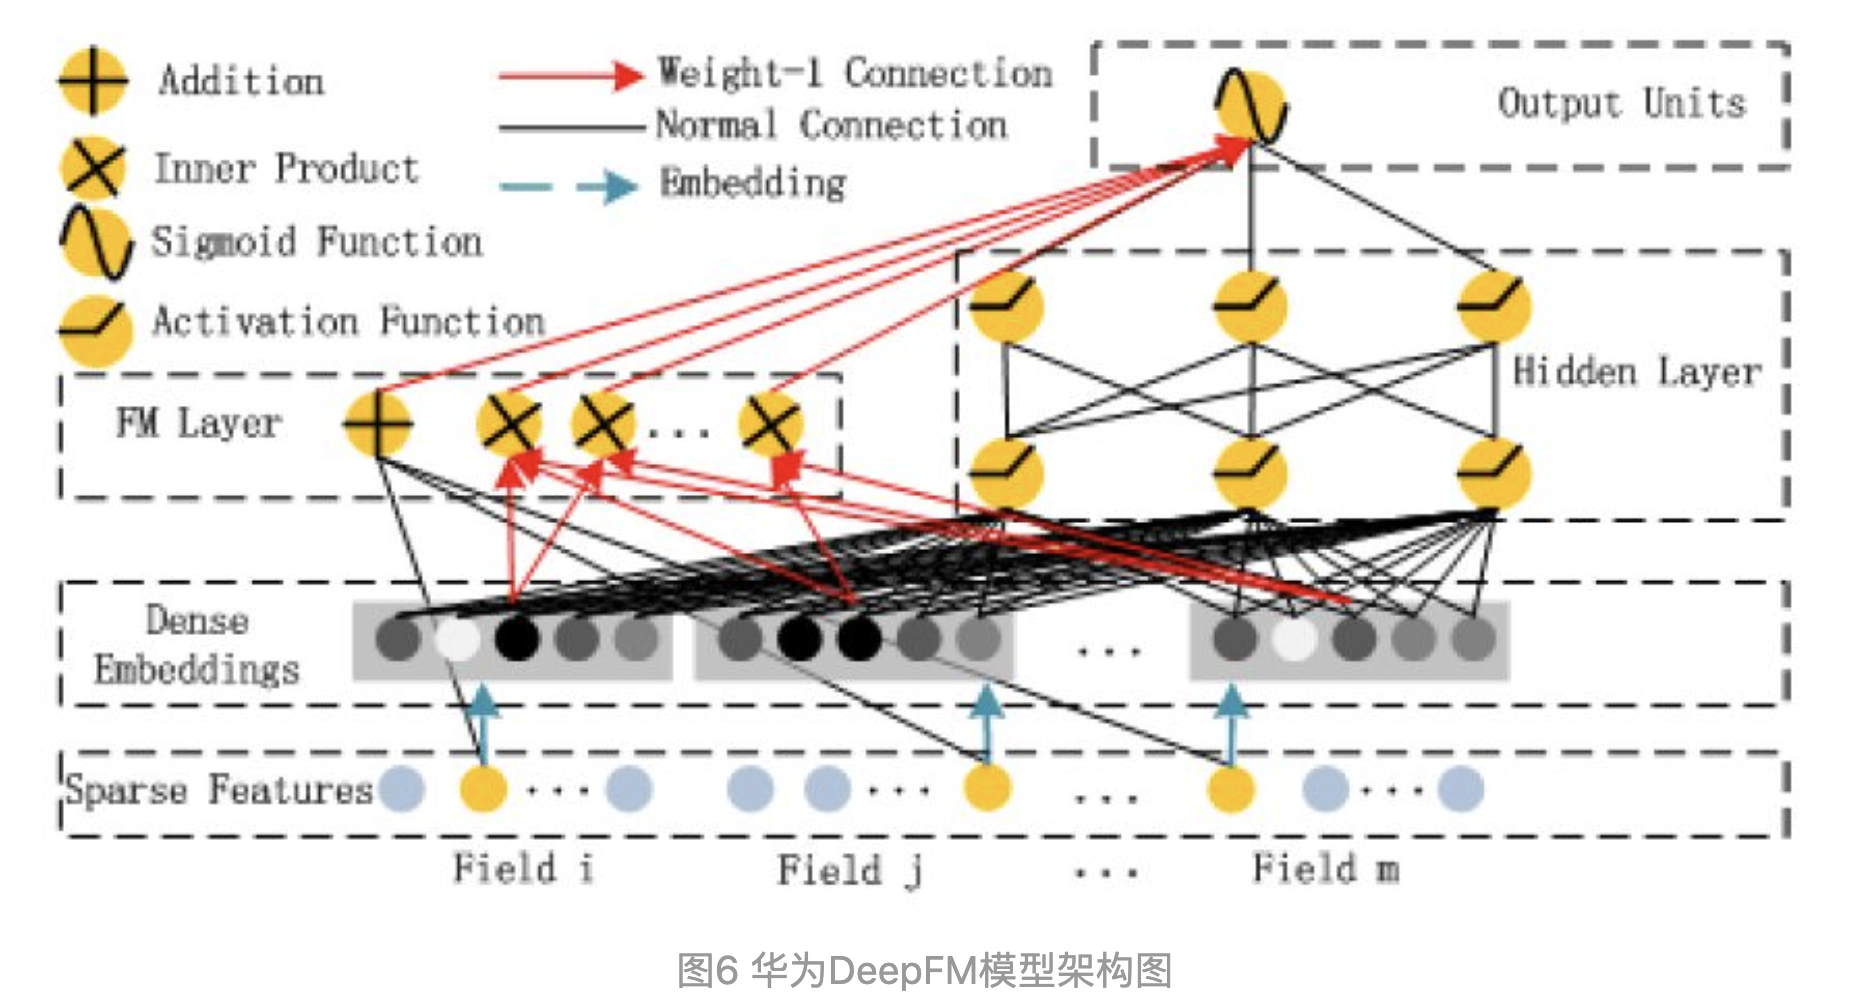
\includegraphics[width=1\textwidth]{fig/Huawei_DeepFM_Structure.png}
\end{figure}

PNN中则是直接加入了Product Layer,加强特征交叉能力。
\begin{figure}[H]
    \centering
    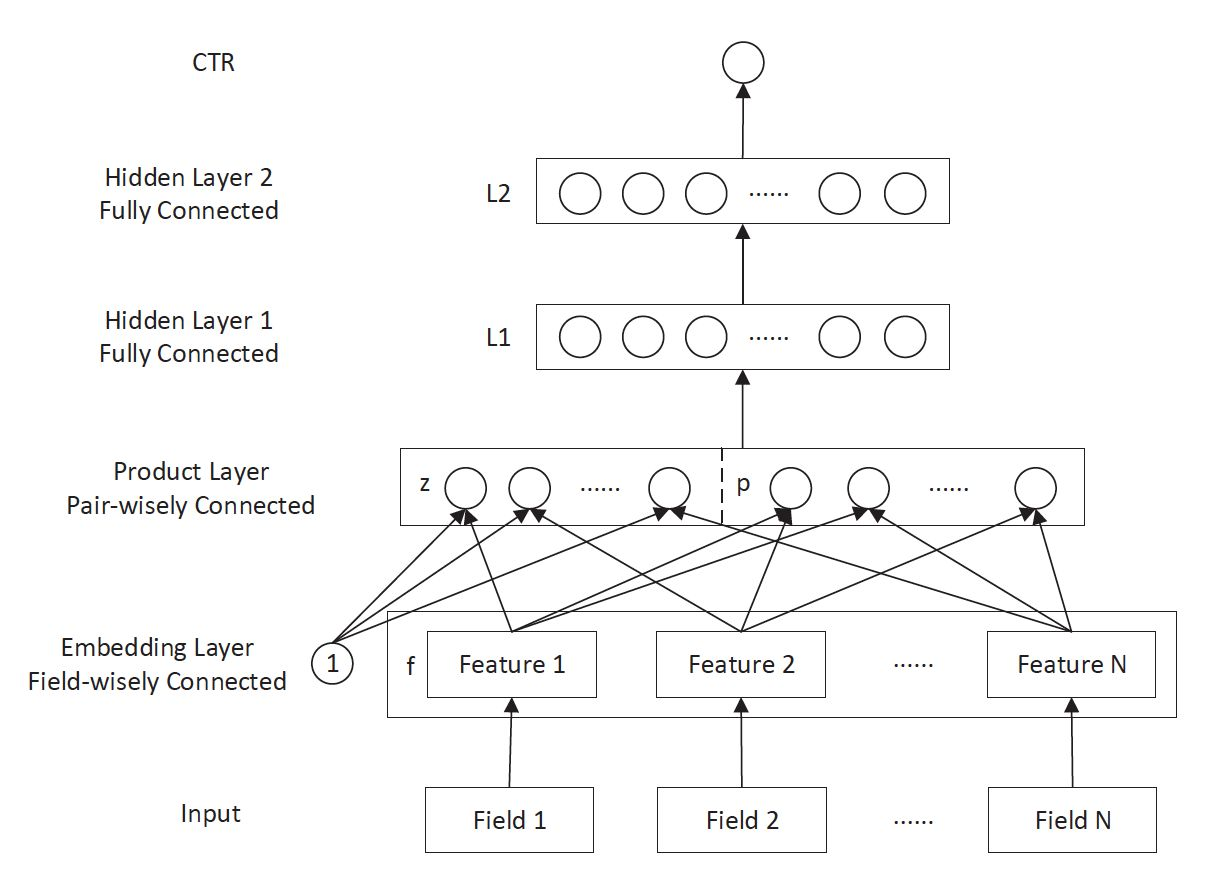
\includegraphics[width=1\textwidth]{fig/PNN_Structure.jpg}
\end{figure}

当然专门针对特征交叉进行改造的模型还有很多,诸如Deep Crossing,Deep\&Cross等。这些网络有的直接通过乘积操作将两个特征相乘,有的通过FM这类善于处理特征交叉的模型作为特征交叉层,有的通过构造一些特征cross的方法进行特征组合。但所有这些都充分说明了一点,仅仅采用MLP进行特征组合的能力是不够的,需要有针对性的在模型中加入特征交叉的结构。

\section{Product 层的具体形式}
Product 层有两种操作形式:Inner Product 和 Outer Product,即内积和外积。

\subsection{Inner Product}
内积操作就是经典的向量内积运算,假设输入特征向量分别为$f_i, f_j$,特征的内积互操作$g_{\text{inner}}(f_i, f_j)$ 的定义为:
$$
g_{\text{inner}}(f_i, f_j) = \langle f_i, f_j \rangle
$$

\subsection{Outer Product}
外积操作是对输入特征向量 $f_i, f_j$ 的各维度进行两两交叉,生成特征交叉矩阵,外积互操作 $g_{\text{outer}}(f_i, f_j)$ 的定义为:
$$
g_{\text{outer}}(f_i, f_j) = f_i f_j^T
$$

外积互操作生成的是特征向量 $f_i, f_j$ 各维度两两交叉而成的一个 $M \times M$ 的方形矩阵(其中 $M$ 是输入向量的维度)。这样的外积操作无疑会将问题的复杂度从原来的 $M$ 提升到了 $M^2$,为了在一定程度上减小模型训练的负担,PNN 模型的论文中介绍了一种降维的方法,就是把所有两两特征 Embedding 向量外积互操作的结果叠加(Superposition),形成一个叠加外积互操作矩阵 $p$,具体定义如下:
$$
p = \sum_{i=1}^N\sum_{j=1}^N g_{\text{outer}}(f_i, f_j) = \sum_{i=1}^N\sum_{j=1}^N f_i f_j^T = f_{\sum}f_{\sum}^T,  \qquad f_{\sum} = \sum_{i=1}^Nf_i
$$

从上式的最终形式来看,叠加矩阵 $p$ 的最终形式类似于让所有特征 Embedding 向量通过一个平均池化层(Average Pooling)后,再进行外积互操作。

在实际应用中,还应对平均池化的操作谨慎对待。因为把不同特征对应维度进行平均,实际上是\textbf{假设不同特征的对应维度具有类似的含义}。但显然,如果一个特征是年龄,另一个特征是地域,那么这两个特征在经过各自的 Embedding 层后,二者的 Embedding 向量不在同一个向量空间中,不具备任何可比性。这时,把二者平均起来,会模糊很多有价值的信息。所以,\textbf{平均池化的操作经常发生在同类 Embedding 上}。例如,将用户浏览过的多个物品的 Embedding 进行平均。同样,这里的 Outer Product 操作也需要谨慎对待。

\section{总结}
MLP理论上具备特征交叉和特征组合的能力,但在神经网络层数较浅时,特征交叉的能力较弱,于是在实践中,往往会在深度学习网络中加入特征交叉的结构来提高特征交叉的效率。




%\printbibliography
\bibliography{../ref}
\bibliographystyle{IEEEtran}
\end{document}
